%\documentclass[10pt,a4paper,final,oneside,openany,article]{memoir}
%\documentclass[letterpaper,a4paper,10pt]{article}
\documentclass[10pt,letterpaper,final]{article}
\usepackage[utf8]{inputenc}
\usepackage[british]{babel}
\usepackage{hyperref}
\setcounter{tocdepth}{3}
\usepackage[draft]{fixme}
\usepackage{abstract}
\usepackage{todonotes}

%% FONT
%\usepackage[T1]{fontenc}
%\usepackage{lmodern}
%\usepackage[urw-garamond]{mathdesign}
% Fonts configuration
%  - Palatino and Bitstream Vera Sans Mono for verbatim
\usepackage[T1]{fontenc}
\usepackage{palatino}
\usepackage[sc]{mathpazo} % Math font for Palatino
\usepackage{bera}
\linespread{1.05} % Palatino needs more leading (space between lines)
\usepackage{microtype}
\usepackage{graphicx} % ++
\usepackage{color}
\definecolor{kugrey}{rgb}{.4,.4,.4}
\usepackage{listings}
\lstset{ %
    language=Python,                % choose the language of the code
    frame=single,                   % adds a frame around the code
    keywordstyle = \textbf,
    commentstyle = \color{kugrey}\textit,
    stringstyle = \ttfamily,
    basicstyle   = \small\ttfamily,
    numberstyle=\tiny,
    sensitive = true,
}

%% odds and ends
%\chapterstyle{hangnum}
\setcounter{secnumdepth}{2}

%HEADINGS
\title{Constructing Models For Diagnosing Rare Diseases\\
        \small{by Using the Google Search Engine}}

\author{Brian S. Mathiasen $-$ soborg@diku.dk \\
        Henrik G. Jensen $-$ henne@diku.dk\\
%        \\
%        Department of Computer Science\\
%        University of Copenhagen\\
%        Universitetsparken 1\\
%        DK-2100 Copenhagen, Denmark
}

\date{\today} %\today

%%
\begin{document}
\maketitle
\listoffixmes
%\tableofcontents


\begin{abstract}
In this paper we design and construct models for assisting physicians
with the task of diagnosing rare diseases. Using a prior knowledge of
rare diseases consisting of \textit{disease name, some symptoms} and
\textit{synonyms}, we utilize the \textit{Google Search Engine} to build
the model over several iterations. The model is constructed using
several machine learning and natural language processing techniques by
text mining symptoms and features from abstracts and other interesting
paragraphs of text found in the search process.

Our tests show that... blablabla, \fxwarning{Abstract, results: to do}
\end{abstract}
%%-----------------------------
%\newpage
\section{Introduction}
\label{chap:introduction}


The structure of this report is as follows:
blablabla... and then some.

\subsection{Limitations}


\section{Previous Work}
Blabla work by radu and paula \cite{radupaula}.


\cite{jensenandersen} proposed a system for diagnosing rare diseases
using vector space models and text mining. They showed a clear potential
in automating such a process, but their results were not statistically
significant. Their system did not rely on prior knowledge of particular
diseases, but still showed that around 60\% of the tests were
satisfactory.


The article \cite{googlingdiagnosis} proves the viability of using
Google as a diagnosis aid, despite the tests being done manually with
little consideration with regard to automation or test reliability and
validity.

%Our system will move on to the next step and introduce intelligent
%automation through a number of predefined criteria and utilizing several
%machine learning and natural language processing techniques.


The editorials \cite{googlechangemedicine} and
\cite{diagnosissearchengines} suggest Google and search engines in
general as being a very strong player in the task of diagnosing
diseases. The witness of search engines being a valuable source of
information is apparent, but the shear amount of misinformation and
noise from regular searches make such a system in it’s current
incarnation unreliable and error prone.
%(Our goal is to refine and provide means for filtering out this noise
%and focus on harvesting information from related material with reference
%to the original search terms as well as specific criteria for the text
%mining process.)


%Inspiration for a system: Online Search Engine specialised for
%diagnosing stuff etc.
%http://www.healthline.com/symptomsearch

%This system is based on simple searches that relies on an already
%established database of diseases with appropriate meta-information. The
%user is able to search for symptoms and can narrow down the search by
%adding several symptoms. The system will then present a list of possible
%diseases according to some relevance criterion.

%(It is an end-user focused system, while our system will be a back-bone
%focused system, attempting to establish a model on which queries may be
%imposed. It will as such automate the information collection based on
%several machine learning and natural language processing techniques
%appropriate for the needs.)


%Google Health: http://www.google.com/intl/en-US/health/about/index.html


%Article by practising doctor on “do’s and don’t’s when using Google as
%diagnosis aid”:
%http://vitualis.wordpress.com/2007/02/26/google-based-medicine/


\section{Method}
As one of the premises of the project was to introduce prior knowledge
of the disease model, we needed to process our available data. We were
given a large corpus of data from Orphanet \ref{app:orphanet},
consisting of \texttt{\{orphanum, disease name, disease
description/abstract, maybe author and date\}} for each disease in the
data set.
The data is processes similar to the method described in
\cite{jensenandersen}, and will thus be used too bootstrap our knowledge
of each disease, allowing us to iterate and harvest additional
information using various harvesting techniques roughly covering the use
of the \textit{Google} search engine to collect an array of websites
given a query relevant to the disease (disease name and a possibly a
number of keywords). For each website, we will collect paragraphs and
save it for further processing if the cosine angle between the two
vectors is within a reasonable threshold. For each accepted paragraph we
use Natural Language Processing (NLP) techniques to identify candidates
for relevant terms and phrases that will then be used to expand the
model. The abstract flow model is available in figure \ref{fig:flow}.


\begin{figure}[htp!]
\begin{center}
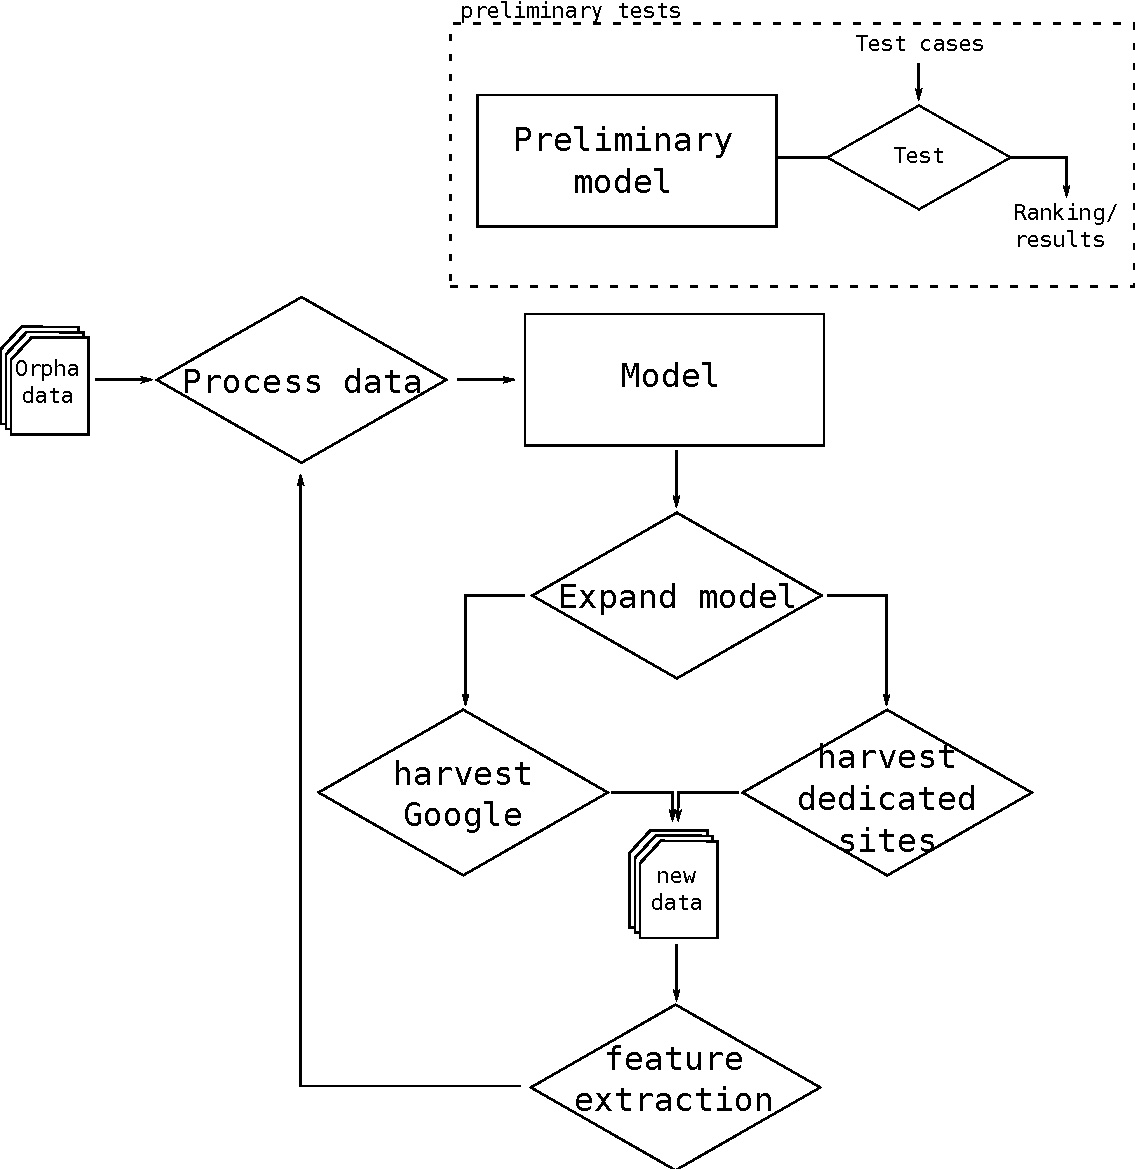
\includegraphics[scale=0.4]{images/pipeline}
\caption{Some crap}
\label{fig:flow}
\end{center}
\end{figure}

The process will be described in greater detail in the following
sections.

\subsection{Building the preliminary model}
\todo[inline]{Explain the construction of the TF-IDF matrix and explain
assumptions for using prior information for harvesting}

\subsection{Harvesting data, or: None Like it Raw!}
\todo[inline]{Explain the technique for googling, including covariance
and relevance measurements. Explain the threshold}

%We will use Natural Language Processing (NLP) techniques to identify
%whether a term or phrase is a symptom.
% E.g. \texttt{thickened blood} is
%a symptom (phrase) while the terms \texttt{thickened} and \texttt{blood}
%on their own are not.

%Our model is based on Machine Learning (ML) clustering algorithms. The
%model, that is trained to classify symptoms into clusters, recognises
%that the majority of those symptoms belong to the cluster of data that
%is associated with one particular disease. This results in a possible
%diagnosis of the disease for the patient, given some level of confidence
%or error.\fxfatal{rewrite or actually implement this clustering wisely!}

%Each cluster within the set of clusters $c \in C$ represents a disease
%which has it's own symptoms that is collected through a prior data-set,
%as provided by OrphanetData \fxfatal{præciser kilden}, and subsequently
%collected through various iterations on search engines and harvested
%using NLP techniques for feature extraction.

%The process is outline as shown below:
%\begin{itemize}
%\item extract features from known abstract
%\item initiate $n$ iterations to harvest more features based on already
%known features and disease meta-data.
%\end{itemize}


\subsection{Feature Extraction}
In order to iterate and collect information to expand the modelling of
relevant terms and phrases we use NLP to identify symptoms and medical
terms (here-on referred to as just symptom) from abstracts and
paragraphs harvested. Identifying unique symptoms and correlate with
other documents describing the same disease will increase the knowledge,
or further substantiate pre-existing knowledge of that disease. The
ultimate goal of this strategy is to expand the model and highlight
unique keywords such that, given our assumption, will increase the
precision of the prediction.

We have observed that symptoms are usually described as zero or more
adjectives or verbs followed by one or more nouns\fxwarning{substantiate this claim somehow}.
Thus we can build a regular grammar using the NLTK library as such:
\begin{lstlisting}
grammar = """CANDIDATE: {VBD><IN>(<SYMPTOM><,|CC>)*}
             SYMPTOM: {<JJ|VB(D|G)>*<NN>+}"""
\end{lstlisting}
This will catch sentences such as \texttt{characterized by s$_{0}$,
s$_{1}$, ... and s$_{n}$}, where \texttt{s$_{i}$} is a potential symptom
candidate.
This will allow us to catch the symptom \texttt{bleeding diathesis}, but
will also match, for our purpose, insignificant medical-related terms
such as \texttt{gene product}.
The premise for the construction of this grammar is substantiated
through anecdotal manual observations of a handful of abstracts from the
orphanet data set, and utilized under the assumption that it will
increase the amount of medically relevant terms as opposed to simply
catching all combinations matching the \texttt{SYMPTOM} grammar above.

\todo[inline]{explain selecting symptoms from databases}

Having collected a number of symptom candidates $\mathbb{S}$ from some
document or paragraph, we calculate number of unique terms and return
the candidates, $\mathbb{S'}$, that appear more than once or a supterm of
other candidates. I.e., consider the candidates $\mathbb{S} = $
\texttt{\{bleeding diathesis, bleeding, sleep apnae\}} we will return
the symptoms $\mathbb{S'} = $ \texttt{\{bleeding diathesis, bleeding\}},
using the mathematical rule:
\begin{equation}
 s_{j}, s_{i} \in \mathbb{S'}\texttt{if count}(s_{j}) > 1 \wedge\texttt{count}(s_{i}) \wedge s_{j} \subset s_{i}, \texttt{for } s_{i}, s_{j} \in \mathbb{S}
\end{equation}
\todo[inline]{valider formel}
Anecdotal observations during the development phase of this module
showed that returning terms and supterms using this mathematical rule
increased the amount of relevant symptoms, and seemed to decrease the
amount of 


\subsubsection{Feature Extraction using NLP}
We will use NLP techniques to extract candidates for this
classification, using Part-of-Speech (POS)
tagging\todo[inline]{Brief explanation here}, and semantic
recognition of terms and phrases.



%After considerable consideration, we have decided to limit the scope of
%our information harvesting to sites, guaranteed to be within the domain
%of disease and/or rare diseases. As such, we methodically crawl each
%known site of interest and extract phrases, paragraphs and documents
%which are suitable candidates to contain information according to the
%query of features.

%While we may potentially lose critical information by limiting our
%searches to specific sites, we also gain precision in our models by only
%harvesting information within our domain. As such, we do not risk
%running into documents that are not necessarily important for the
%purpose of our model, but still show up as a result, caused by more or
%less vague references to the given query. In order to widen the scope of
%the searches, one would have to not only define modular ways of
%extracting valuable information within any site available on the
%Internet, but also look into document classification \cite{Jimmy}, to
%decrease the level of noise. The implementation of such a classification
%model is relatively simple, and only require a substantial amount of
%corpora of documents for training and testing the model, but we did not
%see it as important in this project and will leave the discussion as is.


%For each \texttt{SearchGoogle} instance, we define which domain it
%should retrieve results from, as well as an extractor function that
%reads the results and returns information to be processed further, by
%our feature extraction algorithm. All of these results are thus passed
%into a mathematical model and used to increase disease prediction
%precision or widen the amount of known diseases. I.e. expand the model.


\section{Tests}
\todo[inline]{First some bla.
Then some tables and some more bla!
Investigate possibility of significance testing. How do we fare
mathematically compared to 'Googling for Diagnosis'? Students T-Test or
equiv.}

\subsection{Preliminary Tests}
\todo[inline]{Results and some bla.}


\appendix
\section{Appendix}
\label{app:orphanet}

\renewcommand\bibname{References}
\bibliography{bib}
\bibliographystyle{apalike}

\end{document}
